\documentclass[11pt]{article}
\usepackage[margin=1in]{geometry}
\usepackage{graphicx}
\usepackage{booktabs}
\usepackage{hyperref}
\hypersetup{colorlinks=true,linkcolor=blue,urlcolor=blue}
\title{Episode Tracking Explanation Report}
\author{TP2 SPY Call Pipeline}
\date{June 2026}
\begin{document}
\maketitle

\section*{Why Episode Tracking Exists}
The raw detector output is daily rectangle-level. The same economic TP2
violation can appear on consecutive trading days, so counting every daily row
as an independent ML example would inflate the sample and make train/test
splits less defensible. Episode tracking groups consecutive appearances of the
same left-side pair into one event.

\section*{Episode Key}
The primary key is the left-side pair:
\[
  (A = K_1,T_1), \quad (B = K_2,T_2).
\]
The exact four-leg rectangle, including the rounded adjusted C and D legs, is
also tracked as a diagnostic because forwards and rounded strikes can move
inside the same economic A/B episode.

\section*{Full-Sample Episode Accounting}
\begin{center}
\begin{tabular}{lr}
\toprule
Metric & Value \\
\midrule
Daily violation rows & 2,430,220 \\
Pair episodes & 2,098,213 \\
Unique pair keys & 1,792,462 \\
Single-day episodes & 1,860,180 \\
Single-day episode share & 88.66\% \\
Episodes with exact rectangle changes & 54,996 \\
Median duration & 1 session \\
Maximum duration & 14 sessions \\
\bottomrule
\end{tabular}
\end{center}

\begin{figure}[h]
\centering
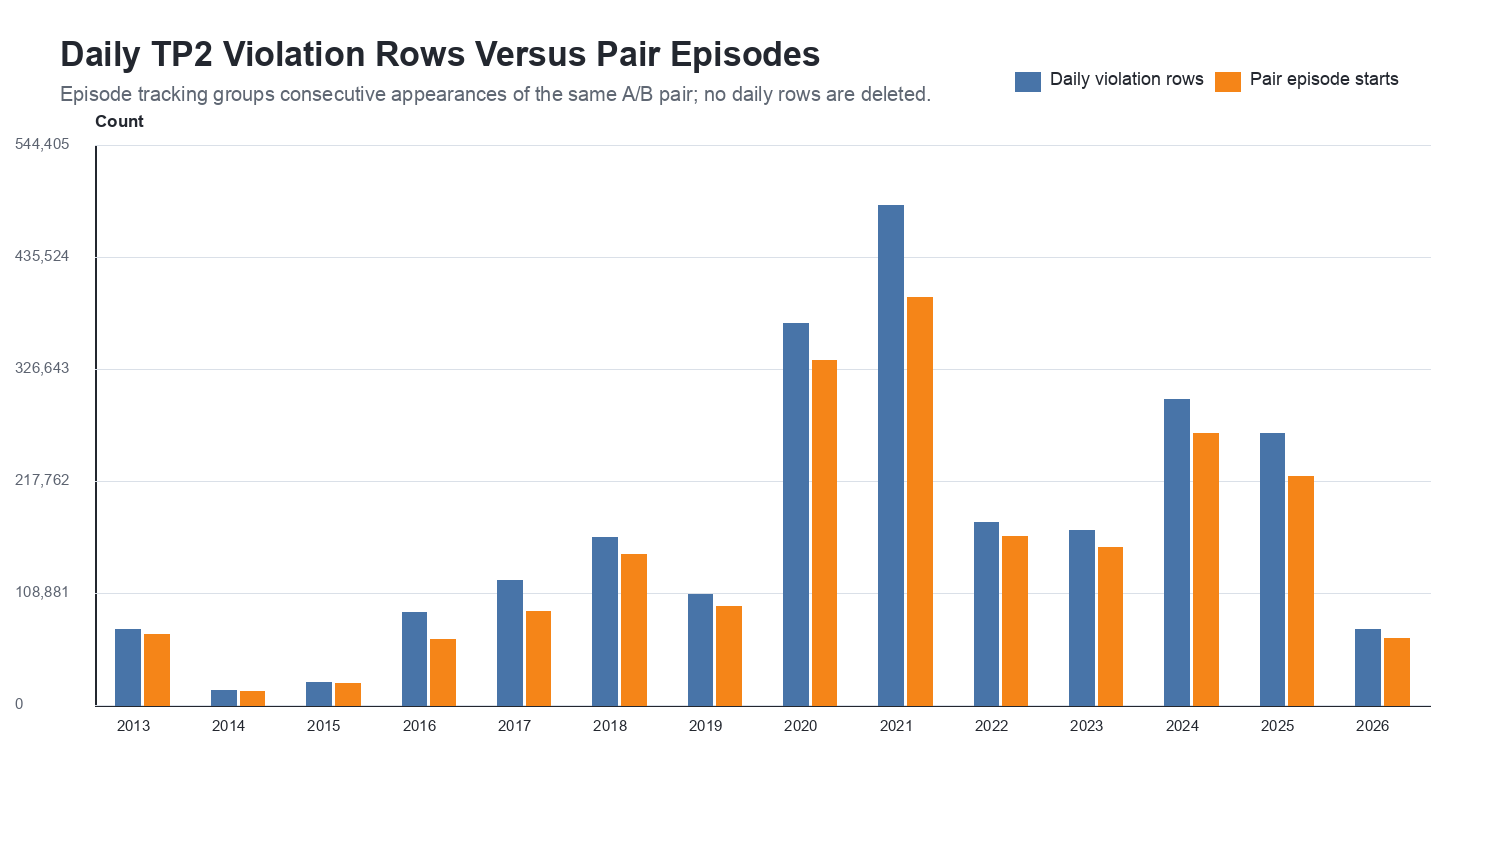
\includegraphics[width=\linewidth]{figures/episode_rows_vs_pair_episodes_by_year.png}
\caption{Daily violation rows versus pair episode starts by year.}
\end{figure}

\begin{figure}[h]
\centering
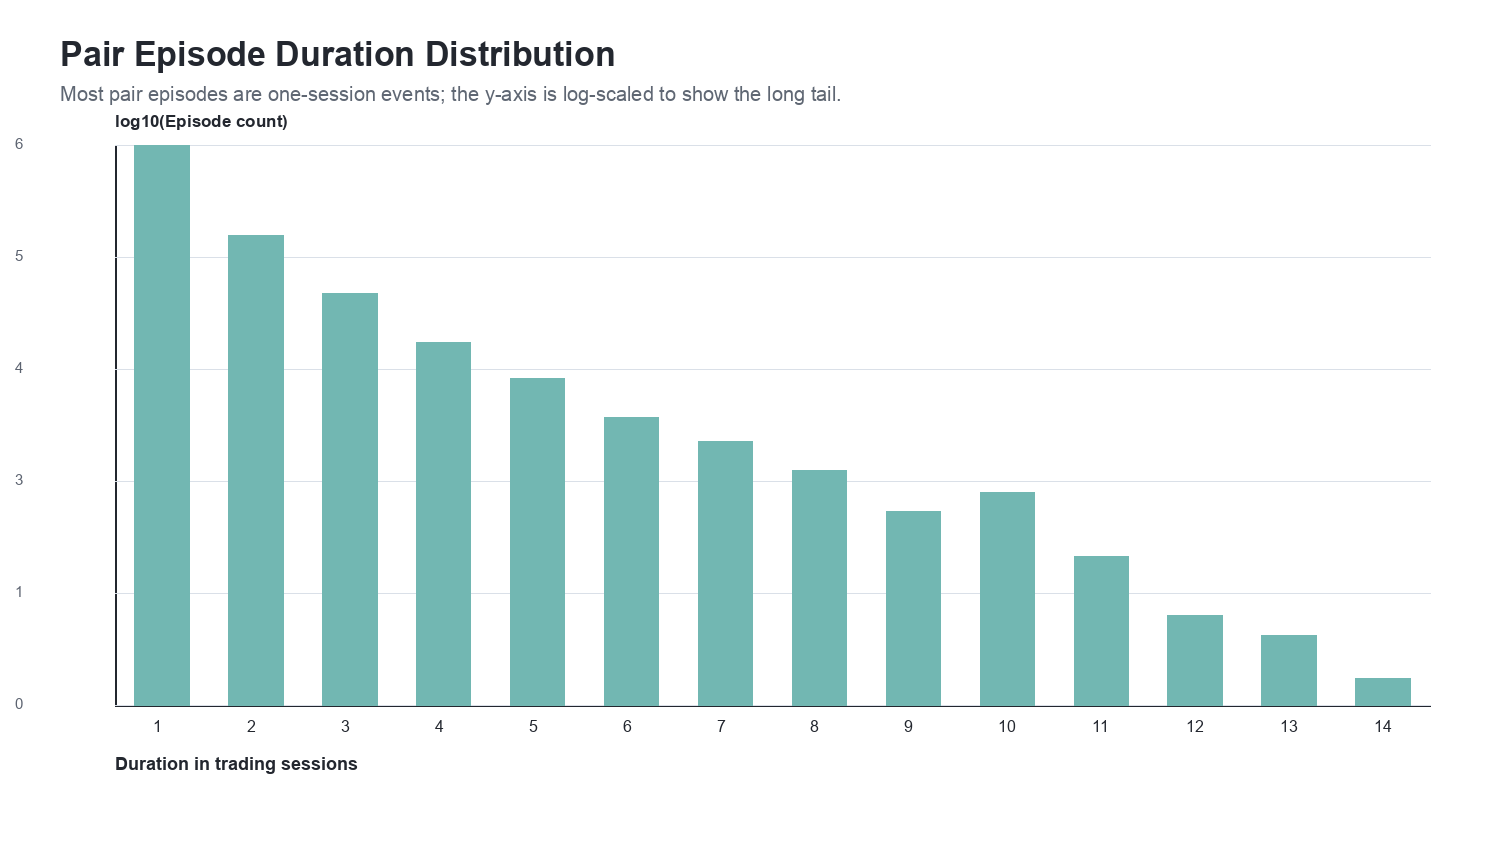
\includegraphics[width=\linewidth]{figures/episode_duration_distribution.png}
\caption{Episode duration distribution. Most episodes last one session.}
\end{figure}

\section*{Interpretation}
Episode tracking is a structural improvement, not just a reporting change. It
makes the ML dataset event-level and avoids repeatedly training on the same
violation while it persists.

\end{document}
